\documentclass{amsart}
\usepackage{amsmath}
\usepackage{graphicx}
\usepackage{booktabs}
\title{Bayesian modeling of COVID-19 epidemic: Japanese case}
\author{Yoriyuki Yamagata}
\address{National Institute of Advanced Industrial Science and Technology (AIST),
1-8-31 Midorigaoka, Ikeda, Japan}
\email{yoriyuki.yamagata@aist.go.jp}
\date{\today}

\begin{document}

\maketitle

\begin{abstract}
 We estimate the daily change of $R$ (the reproducing rate) and reporting rate of COVID-19 infection in Japan by a Bayesian method.
 The estimate reveals a recent downward trend.
 Although our analysis is preliminary, this may suggest that Japanese policy had some impact on the spread of infection.
\end{abstract}

\section{Introduction}

In the wake of the COVID-19 epidemic, the Japanese government gradually employed public health measures against COVID-19.
In the first stage, the stronger quarantine measures at the border were implemented.
Once patients who had no connection to Wuhan appeared inside the border, The government started to track these patients as far as possible and tried to find people contacted to these patients.
Once these ``track and quarantine clusters'' tactics were overwhelmed by the number of patients, the government started to ask ``behavior changes'' to people, culminating ``declaration of the emergency'' on April 6.
Public facilities like libraries were closed.
Large shopping malls and entertainment businesses, such as movie theatres, were asked to be closed.
Restaurants are asked to shorten their operating hours and stop providing alcoholic beverages at night.
Working from home was encouraged, and the citizens were advised to avoid crowded areas and generally avoid going outside unnecessarily.

However, the Japanese legal system does not have enough mechanisms to ``enforce'' these policies.
Thus the effectiveness of these policies is questionable.
Many people are still commuting to their office because many companies lack the necessary ability to allow their employees to work from home.
Many small restaurants and cafes are still running their business because of the lack of financial compensation.

In this paper, we apply a Bayesian method to estimate daily changes of $R0$, which determines the speed of infection, and reporting rate.
The result revealed a recent downward trend of $R0$.
Thus, although our analysis is preliminary, this may indicate that Japanese policy has some effect against COVID-19 infection.
However, the reduction of $R0$ only reaches the level of the minimum achieved around the mid-March, thus it would not be sufficient to prevent the spread of infection yet.

\section{Related works}

Several works employ data-driven methods to predict and measure the public health measure of COVID-19.

Anastassopoulou et al.~\cite{Anastassopoulou2020} apply the SIRD model to Chinese official statistics, estimating parameters using linear regression.
The reporting rate is not estimated from data but assumed.
By these models and parameters, they predict the COVID-19 epidemic in Hubei province.

Diego Caccavo~\cite{Caccavo2020} and independently Peter Turchin~\cite{Turchin2020} apply modified SIRD models, in which parameters change overtime following specific function forms.
Parameters govern these functions are estimated by minimizing the sum-of-square-error.
However, using the sum-of-square method causes over-fitting and always favors a complex model, therefore it is not suitable to access policy effectiveness.
Further, fitting the SIRD model in the early stage of infection is difficult, as pointed out in stat-exchange~\footnote{https://stats.stackexchange.com/questions/446712/fitting-sir-model-with-2019-ncov-data-doesnt-conververge}.
Using a Bayesian method, we avoid these problems to some degree, because a Bayesian method estimates parameter distribution instead of a point estimate.
Thus, we can assess the degree of confidence of each parameter.
Further, by well-established statistical methods, we can compare the explanatory power of different models.

Flaxman et al.~\cite{Flaxman2020} use a Bayesian model to estimate policy effectiveness.
The methodology is different from us because they assume immediate effects from the policies implemented.
Further, they use a discrete renewal process, a more advanced model than the SIRD model.
They use parameters estimated from studies of clinical cases while we use a purely data-driven method.

\section{Method and materials}

\subsection{Model}

We use the discrete-time SIRD model but assume that the number of move between each category is stochastic and follows Poisson distribution.

\begin{align}
 NI(t) &\sim \textup{Poisson}(\frac{\beta I S}{P})\\
 NR(t) &\sim \textup{Poisson}(\gamma I)\\
 ND(t) &\sim \textup{Poisson}(\delta I)\\
 I(t+1) &= I(t) + NI(t) - NR(t) - ND(t)\\
 S(t+1) &= S(t) - NI(t)\\
 R(t+1) &= R(t) + NR(t)\\
 D(t+1) &= D(t) + ND(t)
\end{align}
The effective reproduction rate can be written
\begin{equation}
    R = \frac{\beta}{\gamma + \delta} \cdot \frac{S}{P}
\end{equation}
When $R$ becomes $<1$ then the infection starts to decline.

We cannot expect that these values are directly observable, because many (or most) cases are mild or asymptomatic.
Therefore, we introduce the reporting rate $q$ and let the number of cumulative observed cases $C_{\text{obs}}$, recovered $R_{\text{obs}}$ and death $D_{\text{obs}}$ as
\begin{align}
 NI_{\text{obs}}(t+1) &\sim \textup{Poisson}(q NI(t))\\
 NR_{\text{obs}}(t+1) &\sim \textup{Poisson}(\gamma I_{\text{obs}}(t))\\
 ND_{\text{obs}}(t+1) &\sim \textup{Poisson}(\delta I_{\text{obs}}(t))\\
 I_{\text{obs}}(t+1) &= I_{\text{obs}}(t) + NI_{\text{obs}}(t+1) - NR_{\text{obs}}(t+1) - ND_{\text{obs}}(t+1)\\
 R_{\text{obs}}(t+1) &= R_{\text{obs}}(t) + NR_{\text{obs}}(t)\\
 D_{\text{obs}}(t+1) &= D_{\text{obs}}(t) + ND_{\text{obs}}(t)
\end{align}

We assume that $\beta$ and $q$ change day to day bases while other parameters are fixed.
To get a reasonable estimate, we assume prior distributions somewhat arbitrary chosen.
\begin{gather}
 S(0) = I(0) \sim \textup{Student\_t}(3, 0, 1)\\
 \beta(0) \sim \textup{Student\_t}(3, 0, 1)\\
 q(0) \sim \textup{Beta}(1, 1)\\
 \beta(t+1) \sim \textup{Student\_t}(3, \beta(t), \sigma_b)\\
 q(t+1) \sim \textup{Beta}(\alpha_q q(t), \alpha_q(1 - q(t)))
\end{gather}
where $\sigma_b \sim \textup{Gamma}(1, 1)$ and $\alpha_q \sim \textup{Gamma}(1, 1)$.
To make our model robust, we choose Student-t as a prior for $\beta$.

% \subsection{Implementation}

% We used Stan~\cite{carpenter2017stan} for Bayesian modeling and parameter inference.
% Inferred data was processed ArviZ~\cite{arviz_2019}.
% Pandas~\cite{reback2020pandas} and xarray~\cite{hoyer2017xarray} were used for pre- and post-data processing.
% Seaborn~\footnote{https://seaborn.pydata.org} was used for visualization.

\subsection{Experiment}

Data up to April 29 were drawn from data repository~\footnote{https://github.com/CSSEGISandData/COVID-19} by Johns Hopkins University Center for Systems Science and Engineering.
Nation-wide numbers of confirmed cases, recovered cases and death were obtained.

These data were fed to Stan~\cite{carpenter2017stan} for Bayesian modeling and parameter inference.
We simplified our model to easy modeling in Stan.
Because latent discrete variables cannot be used in Stan, we used real numbers for $NI(t), NR(t)$ and $ND(t)$.
We used normal approximation $\mathcal{N}(\lambda, \sqrt{\lambda})$ for the Poisson distribution used for $NI(t)$.
For $NR(t)$ and $ND(t)$, we replaced stochastic laws to deterministic laws
\begin{align}
 NR(t) &= \gamma I\\
 ND(t) &= \delta I
\end{align}
to avoid a numerical issue.

Parameter estimation used 2,000 iterations with 1,000 iterations for warm-up and 1,000 iterations for sampling.
Four (default number of Stan) independent computations were performed simultaneously and used to check convergence.
$\hat{R}$~\cite{vehtari2019rank}, which measures convergence, were excellent, within $\hat{R} < 1.1$ for all parameters. 

To make sure that our results are meaningful, we compared the performance of our model with a model (we refer it by ``the constant model''), which assumes constant $\beta$ and $q$.
Parameters were estimated for the constant model in the same way and LOO-CV, a standard measure of model performance, was compared.
Because the exact computation of LOO-CV is computationally expensive, approximation PSIS-LOO-CV~\cite{Vehtari2017} and WAIC~\cite{watanabe2010asymptotic} were compared (Table~\ref{tbl:IC}).
Our model outperforms the constant model respect to both measures.
However, the tool reported high Pareto-k for the importance weight distribution, which indicates that the model is not robust and parameter estimate depends too much on specific data points.
In such a case, both measure is not very reliable.


\begin{table}[h]
\begin{center}
\begin{tabular}{lrr} \toprule
Model & PSIS-LOO & WAIC \\ \midrule 
Const & 3440.36 &  4659.53 \\ 
Daily Change & 685.53 & 634.754 \\
\bottomrule\\
\end{tabular}
\caption{Comparison of PSIS-LOO and WAIC for each model.  Const is the model with fixed $\beta$ and the reporting rate while Daily Change allows daily changes.  A model with a smaller score is better.}
\label{tbl:IC}
\end{center}
\end{table}

Models and the computation history used for this experiment are public at GitHub~\footnote{https://github.com/yoriyuki/BayesianCOVID19/tree/used-for-paper-v2/notebook}.

\section{Results}

Fig.~\ref{fig:b} shows an estimated $R$ for each day.
Because the Bayesian estimation gives a distribution of parameters, the lower (25\% percentile) estimate is shown by a dotted green line, the median estimate is shown by a solid blue line and the upper (75\% percentile) is shown a broken orange line.
\begin{figure}[h]
 \centering
 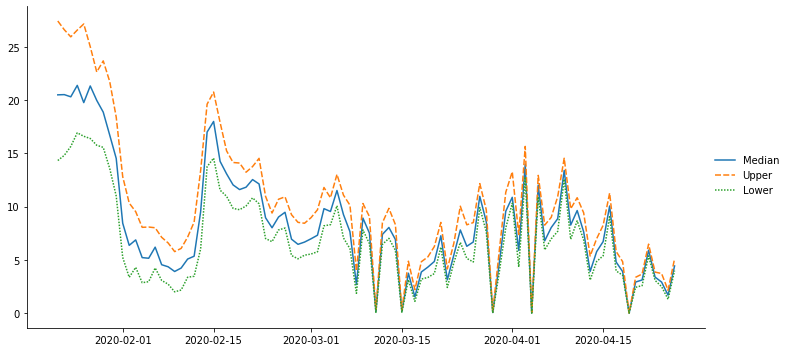
\includegraphics[width=\linewidth]{fig/R-Japan.png}
 \caption{ change over time of $R$}
 \label{fig:b}
\end{figure}
The first downward trend may not be very reliable because there is a few data for infection.
The downward trend from the mid. February trend until the mid. March could be explained by public awareness and tracking effort of infection.
After the mid. March, the tracking effort might be overwhelmed, thus created an upward trend until the beginning of April, when ``the state of emergency'' was declared to major urban areas.
Since then, there was a slow downward trend, but it is unclear how long it will continue.
It appears that ``the state of emergency'' only achieved the minimum $R$ achieved around the mid. March so far and still larger than 0.
Therefore, we can predict that the infection will sill expand in future.

\begin{figure}[h]
 \centering
 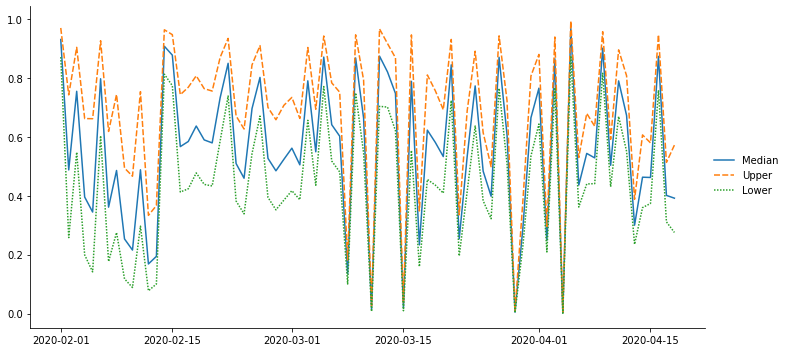
\includegraphics[width=\linewidth]{fig/q-Japan.png}
 \caption{Change over time of the reporting rate $q$}
 \label{fig:q}
\end{figure}

Fig.~\ref{fig:q} shows an estimated reporting rate.
The result is very noisy.
It could suggest that the reported number is strongly influenced by reporting practice.

We compare the result with Korea (Fig.~\ref{fig:R-China}) and China (Fig.~\ref{fig:R-Korea}).
\begin{figure}[h]
    \centering
    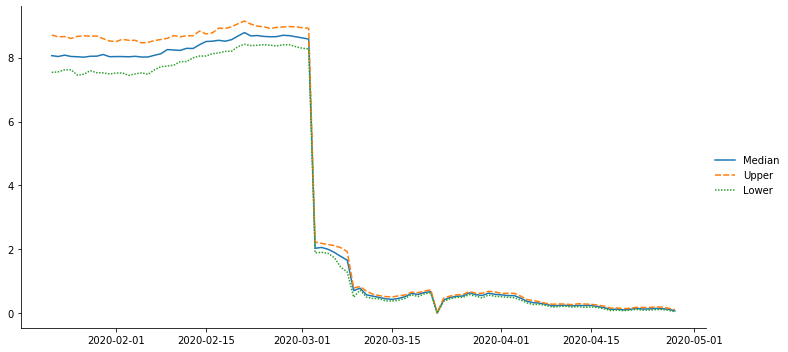
\includegraphics[width=\linewidth]{fig/R-Korea.png}
    \caption{ change over time of $R$ in Korea}
    \label{fig:R-Korea}
\end{figure}
\begin{figure}[h]
    \centering
    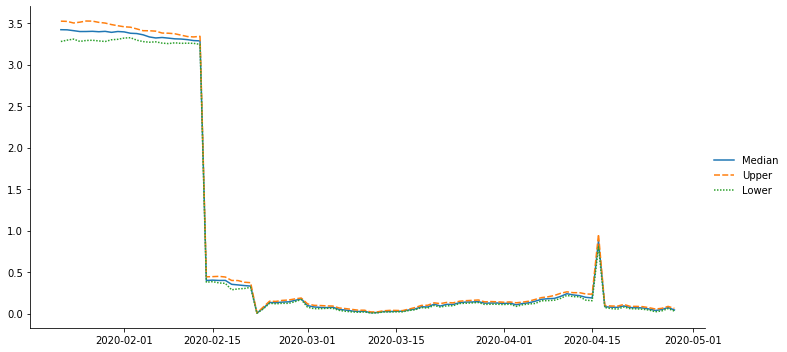
\includegraphics[width=\linewidth]{fig/R-China.png}
    \caption{ change over time of $R$ in China}
    \label{fig:R-China}
\end{figure}
Both show excellent convergence ($\hat{R}$) and model selection favors the daily-change model over the constant model.
Both indicate clear downward trend and now $R < 1$, showing these countries are about exiting from the epidemic.

We also applied our method to Italy, for which the our method did not converge, and Pakistan, for which we need to exclude the data until Mar 1, 2020 to achieve convergence.
Therefore, the results of these countries are not shown here.
   
\section{Discussion}

There is a lot of room for improvement.
First, the sensitivity analysis of Bayesian priors would be required.
We often encounter non-convergence for different data set and slightly different prior distribution, indicating non-robustness of our model.
For reliable results, improvement of robustness would be required.
Also, the use of PSI-LOO-CV and WAIC for model selection needs to be reconsidered, because both measure the model's prediction capability, but our goal is not a prediction.

\section*{Acknowledgement}

The author thanks to Kentaro Matsura and the Tokyo.R Slack group for many suggestions and advices on Bayesian modeling.
The author also thanks to Peter Turchin, from whose work the author's work started.

\bibliographystyle{plain}
\bibliography{BayesianCOVID-19}

\end{document}